\begin{frame}{Exemplo de inserção utilizando encadeamento}

    \begin{figure}
        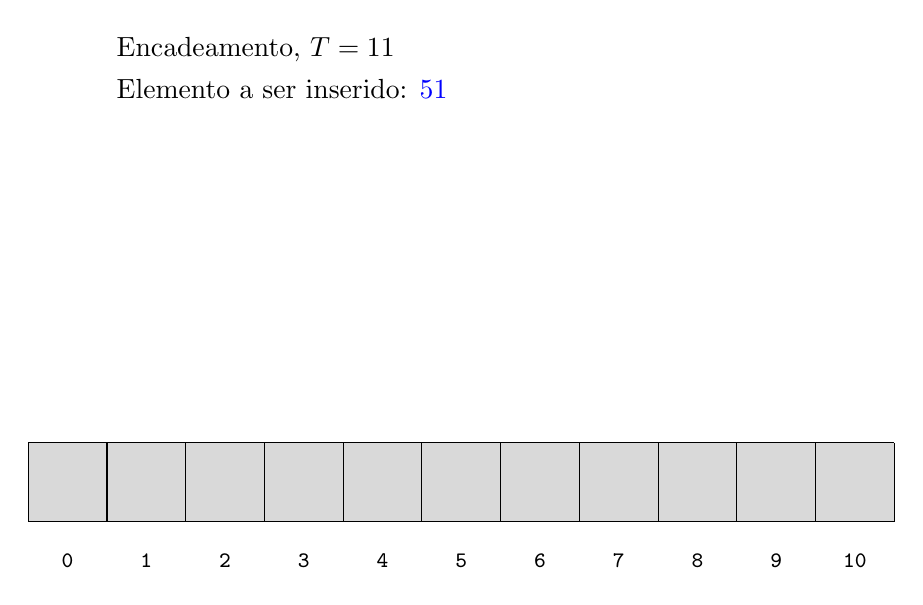
\begin{tikzpicture}
            \fill[gray!30] (0, 1) rectangle (11, 2);
            \draw (0, 1) grid (11, 2);

            \node at (0.5, 0.5) { \tt \footnotesize 0 };
            \node at (1.5, 0.5) { \tt \footnotesize 1 };
            \node at (2.5, 0.5) { \tt \footnotesize 2 };
            \node at (3.5, 0.5) { \tt \footnotesize 3 };
            \node at (4.5, 0.5) { \tt \footnotesize 4 };
            \node at (5.5, 0.5) { \tt \footnotesize 5 };
            \node at (6.5, 0.5) { \tt \footnotesize 6 };
            \node at (7.5, 0.5) { \tt \footnotesize 7 };
            \node at (8.5, 0.5) { \tt \footnotesize 8 };
            \node at (9.5, 0.5) { \tt \footnotesize 9 };
            \node at (10.5, 0.5) { \tt \footnotesize 10 };

            \node[anchor=west] at (1, 7) { Encadeamento, $T = 11$ };
            \node[anchor=west] at (1, 6.5) { Elemento a ser inserido: \textcolor{blue}{$51$} };

        \end{tikzpicture}
    \end{figure}

\end{frame}

\begin{frame}{Exemplo de inserção utilizando encadeamento}

    \begin{figure}
        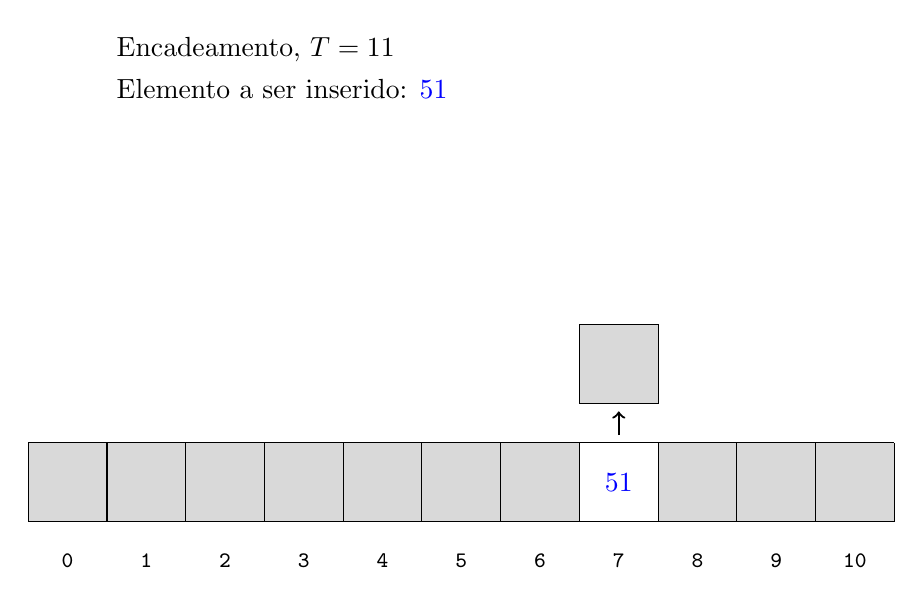
\begin{tikzpicture}
            \fill[gray!30] (0, 1) rectangle (11, 2);
            \draw[fill=white] (7, 1) rectangle (8, 2);
            \draw (0, 1) grid (11, 2);

            \node at (0.5, 0.5) { \tt \footnotesize 0 };
            \node at (1.5, 0.5) { \tt \footnotesize 1 };
            \node at (2.5, 0.5) { \tt \footnotesize 2 };
            \node at (3.5, 0.5) { \tt \footnotesize 3 };
            \node at (4.5, 0.5) { \tt \footnotesize 4 };
            \node at (5.5, 0.5) { \tt \footnotesize 5 };
            \node at (6.5, 0.5) { \tt \footnotesize 6 };
            \node at (7.5, 0.5) { \tt \footnotesize 7 };
            \node at (8.5, 0.5) { \tt \footnotesize 8 };
            \node at (9.5, 0.5) { \tt \footnotesize 9 };
            \node at (10.5, 0.5) { \tt \footnotesize 10 };

            \draw[->, thick] (7.5, 2.1) -- (7.5, 2.4);
            \draw[fill=gray!30] (7, 2.5) rectangle (8, 3.5);
            \node at (7.5, 1.5) { \textcolor{blue}{$51$} };

            \node[anchor=west] at (1, 7) { Encadeamento, $T = 11$ };
            \node[anchor=west] at (1, 6.5) { Elemento a ser inserido: \textcolor{blue}{$51$} };

        \end{tikzpicture}
    \end{figure}

\end{frame}

\begin{frame}{Exemplo de inserção utilizando encadeamento}

    \begin{figure}
        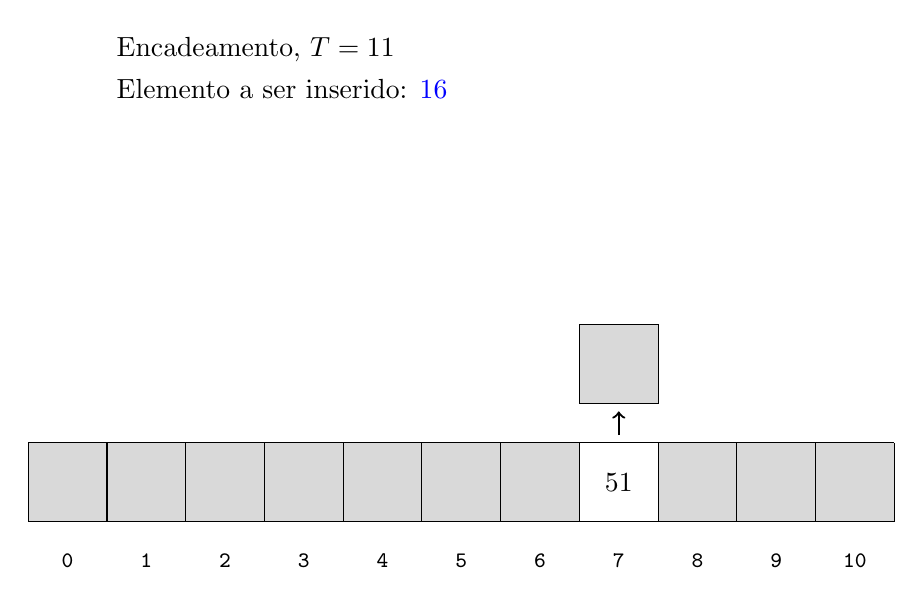
\begin{tikzpicture}
            \fill[gray!30] (0, 1) rectangle (11, 2);
            \draw[fill=white] (7, 1) rectangle (8, 2);
            \draw (0, 1) grid (11, 2);

            \node at (0.5, 0.5) { \tt \footnotesize 0 };
            \node at (1.5, 0.5) { \tt \footnotesize 1 };
            \node at (2.5, 0.5) { \tt \footnotesize 2 };
            \node at (3.5, 0.5) { \tt \footnotesize 3 };
            \node at (4.5, 0.5) { \tt \footnotesize 4 };
            \node at (5.5, 0.5) { \tt \footnotesize 5 };
            \node at (6.5, 0.5) { \tt \footnotesize 6 };
            \node at (7.5, 0.5) { \tt \footnotesize 7 };
            \node at (8.5, 0.5) { \tt \footnotesize 8 };
            \node at (9.5, 0.5) { \tt \footnotesize 9 };
            \node at (10.5, 0.5) { \tt \footnotesize 10 };

            \draw[->, thick] (7.5, 2.1) -- (7.5, 2.4);
            \draw[fill=gray!30] (7, 2.5) rectangle (8, 3.5);
            \node at (7.5, 1.5) { \textcolor{black}{$51$} };

            \node[anchor=west] at (1, 7) { Encadeamento, $T = 11$ };
            \node[anchor=west] at (1, 6.5) { Elemento a ser inserido: \textcolor{blue}{$16$} };

        \end{tikzpicture}
    \end{figure}

\end{frame}

\begin{frame}{Exemplo de inserção utilizando encadeamento}

    \begin{figure}
        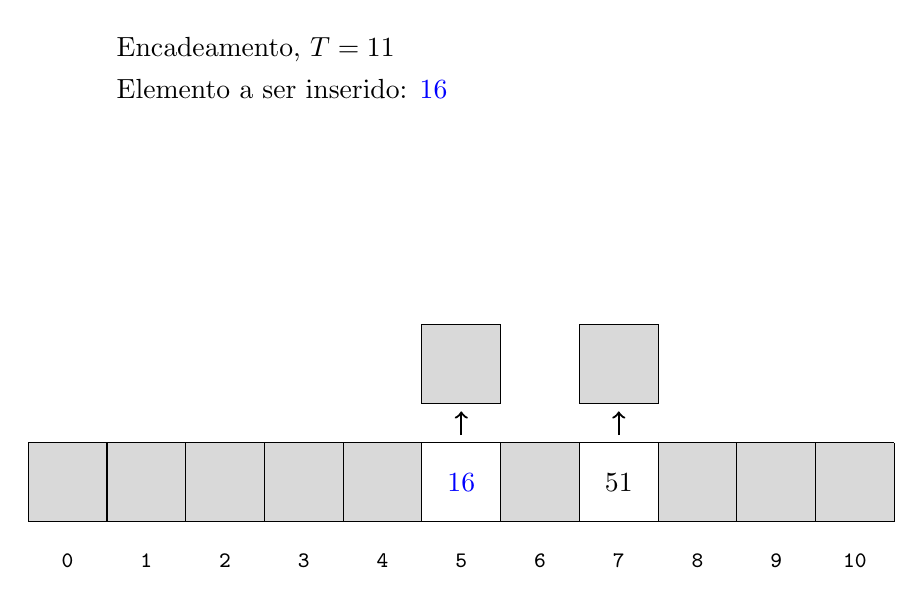
\begin{tikzpicture}
            \fill[gray!30] (0, 1) rectangle (11, 2);
            \draw[fill=white] (7, 1) rectangle (8, 2);
            \draw[fill=white] (5, 1) rectangle (6, 2);
            \draw (0, 1) grid (11, 2);

            \node at (0.5, 0.5) { \tt \footnotesize 0 };
            \node at (1.5, 0.5) { \tt \footnotesize 1 };
            \node at (2.5, 0.5) { \tt \footnotesize 2 };
            \node at (3.5, 0.5) { \tt \footnotesize 3 };
            \node at (4.5, 0.5) { \tt \footnotesize 4 };
            \node at (5.5, 0.5) { \tt \footnotesize 5 };
            \node at (6.5, 0.5) { \tt \footnotesize 6 };
            \node at (7.5, 0.5) { \tt \footnotesize 7 };
            \node at (8.5, 0.5) { \tt \footnotesize 8 };
            \node at (9.5, 0.5) { \tt \footnotesize 9 };
            \node at (10.5, 0.5) { \tt \footnotesize 10 };

            \draw[->, thick] (7.5, 2.1) -- (7.5, 2.4);
            \draw[fill=gray!30] (7, 2.5) rectangle (8, 3.5);
            \node at (7.5, 1.5) { \textcolor{black}{$51$} };

            \draw[->, thick] (5.5, 2.1) -- (5.5, 2.4);
            \draw[fill=gray!30] (5, 2.5) rectangle (6, 3.5);
            \node at (5.5, 1.5) { \textcolor{blue}{$16$} };

            \node[anchor=west] at (1, 7) { Encadeamento, $T = 11$ };
            \node[anchor=west] at (1, 6.5) { Elemento a ser inserido: \textcolor{blue}{$16$} };

        \end{tikzpicture}
    \end{figure}

\end{frame}

\begin{frame}{Exemplo de inserção utilizando encadeamento}

    \begin{figure}
        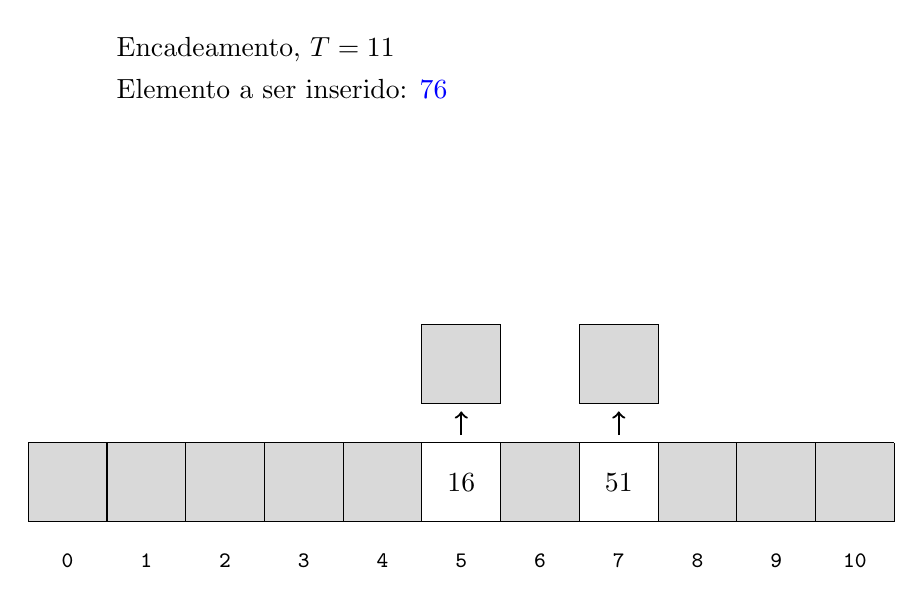
\begin{tikzpicture}
            \fill[gray!30] (0, 1) rectangle (11, 2);
            \draw[fill=white] (7, 1) rectangle (8, 2);
            \draw[fill=white] (5, 1) rectangle (6, 2);
            \draw (0, 1) grid (11, 2);

            \node at (0.5, 0.5) { \tt \footnotesize 0 };
            \node at (1.5, 0.5) { \tt \footnotesize 1 };
            \node at (2.5, 0.5) { \tt \footnotesize 2 };
            \node at (3.5, 0.5) { \tt \footnotesize 3 };
            \node at (4.5, 0.5) { \tt \footnotesize 4 };
            \node at (5.5, 0.5) { \tt \footnotesize 5 };
            \node at (6.5, 0.5) { \tt \footnotesize 6 };
            \node at (7.5, 0.5) { \tt \footnotesize 7 };
            \node at (8.5, 0.5) { \tt \footnotesize 8 };
            \node at (9.5, 0.5) { \tt \footnotesize 9 };
            \node at (10.5, 0.5) { \tt \footnotesize 10 };

            \draw[->, thick] (7.5, 2.1) -- (7.5, 2.4);
            \draw[fill=gray!30] (7, 2.5) rectangle (8, 3.5);
            \node at (7.5, 1.5) { \textcolor{black}{$51$} };

            \draw[->, thick] (5.5, 2.1) -- (5.5, 2.4);
            \draw[fill=gray!30] (5, 2.5) rectangle (6, 3.5);
            \node at (5.5, 1.5) { \textcolor{black}{$16$} };

            \node[anchor=west] at (1, 7) { Encadeamento, $T = 11$ };
            \node[anchor=west] at (1, 6.5) { Elemento a ser inserido: \textcolor{blue}{$76$} };

        \end{tikzpicture}
    \end{figure}

\end{frame}

\begin{frame}{Exemplo de inserção utilizando encadeamento}

    \begin{figure}
        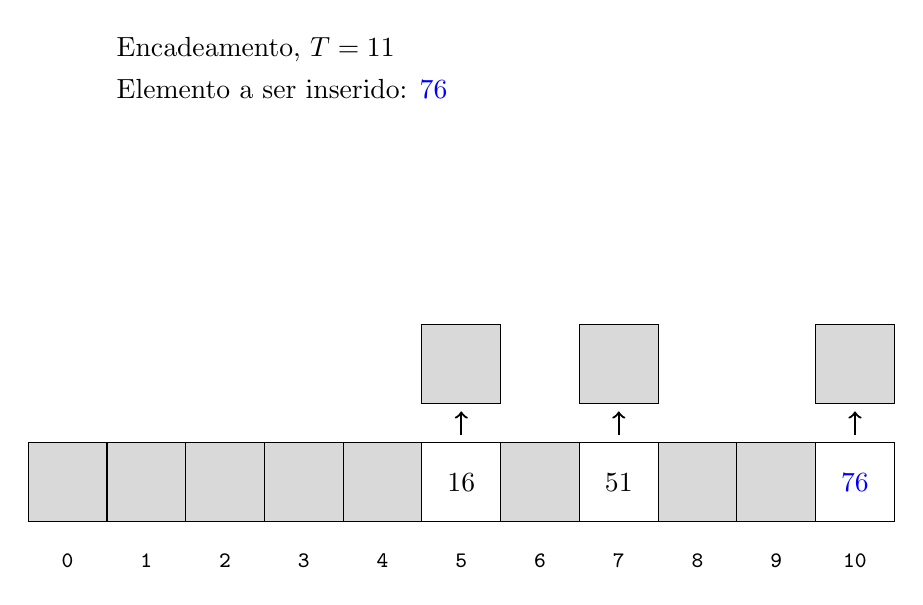
\begin{tikzpicture}
            \fill[gray!30] (0, 1) rectangle (11, 2);
            \draw[fill=white] (7, 1) rectangle (8, 2);
            \draw[fill=white] (5, 1) rectangle (6, 2);
            \draw[fill=white] (10, 1) rectangle (11, 2);
            \draw (0, 1) grid (11, 2);

            \node at (0.5, 0.5) { \tt \footnotesize 0 };
            \node at (1.5, 0.5) { \tt \footnotesize 1 };
            \node at (2.5, 0.5) { \tt \footnotesize 2 };
            \node at (3.5, 0.5) { \tt \footnotesize 3 };
            \node at (4.5, 0.5) { \tt \footnotesize 4 };
            \node at (5.5, 0.5) { \tt \footnotesize 5 };
            \node at (6.5, 0.5) { \tt \footnotesize 6 };
            \node at (7.5, 0.5) { \tt \footnotesize 7 };
            \node at (8.5, 0.5) { \tt \footnotesize 8 };
            \node at (9.5, 0.5) { \tt \footnotesize 9 };
            \node at (10.5, 0.5) { \tt \footnotesize 10 };

            \draw[->, thick] (7.5, 2.1) -- (7.5, 2.4);
            \draw[fill=gray!30] (7, 2.5) rectangle (8, 3.5);
            \node at (7.5, 1.5) { \textcolor{black}{$51$} };

            \draw[->, thick] (5.5, 2.1) -- (5.5, 2.4);
            \draw[fill=gray!30] (5, 2.5) rectangle (6, 3.5);
            \node at (5.5, 1.5) { \textcolor{black}{$16$} };

            \draw[->, thick] (10.5, 2.1) -- (10.5, 2.4);
            \draw[fill=gray!30] (10, 2.5) rectangle (11, 3.5);
            \node at (10.5, 1.5) { \textcolor{blue}{$76$} };

            \node[anchor=west] at (1, 7) { Encadeamento, $T = 11$ };
            \node[anchor=west] at (1, 6.5) { Elemento a ser inserido: \textcolor{blue}{$76$} };

        \end{tikzpicture}
    \end{figure}

\end{frame}

\begin{frame}{Exemplo de inserção utilizando encadeamento}

    \begin{figure}
        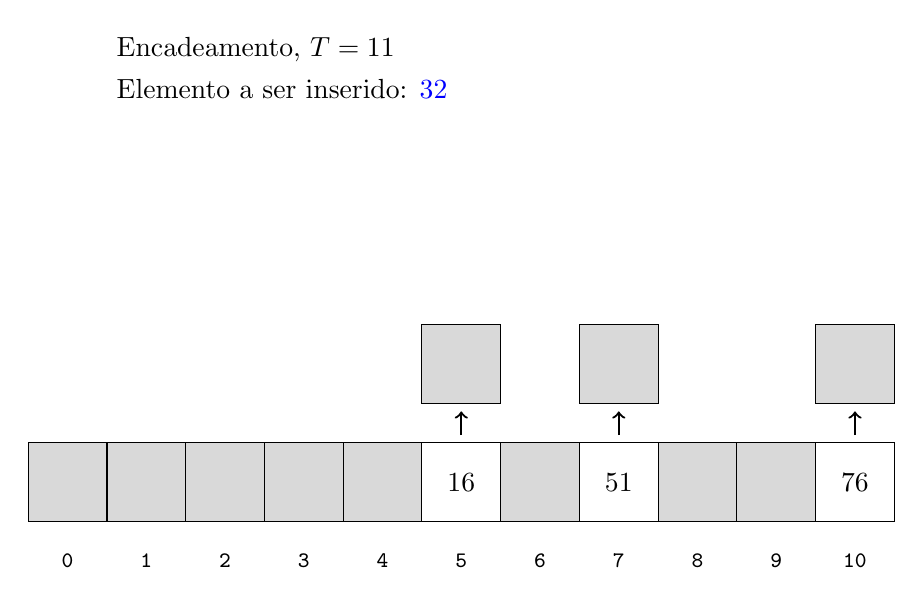
\begin{tikzpicture}
            \fill[gray!30] (0, 1) rectangle (11, 2);
            \draw[fill=white] (7, 1) rectangle (8, 2);
            \draw[fill=white] (5, 1) rectangle (6, 2);
            \draw[fill=white] (10, 1) rectangle (11, 2);
            \draw (0, 1) grid (11, 2);

            \node at (0.5, 0.5) { \tt \footnotesize 0 };
            \node at (1.5, 0.5) { \tt \footnotesize 1 };
            \node at (2.5, 0.5) { \tt \footnotesize 2 };
            \node at (3.5, 0.5) { \tt \footnotesize 3 };
            \node at (4.5, 0.5) { \tt \footnotesize 4 };
            \node at (5.5, 0.5) { \tt \footnotesize 5 };
            \node at (6.5, 0.5) { \tt \footnotesize 6 };
            \node at (7.5, 0.5) { \tt \footnotesize 7 };
            \node at (8.5, 0.5) { \tt \footnotesize 8 };
            \node at (9.5, 0.5) { \tt \footnotesize 9 };
            \node at (10.5, 0.5) { \tt \footnotesize 10 };

            \draw[->, thick] (7.5, 2.1) -- (7.5, 2.4);
            \draw[fill=gray!30] (7, 2.5) rectangle (8, 3.5);
            \node at (7.5, 1.5) { \textcolor{black}{$51$} };

            \draw[->, thick] (5.5, 2.1) -- (5.5, 2.4);
            \draw[fill=gray!30] (5, 2.5) rectangle (6, 3.5);
            \node at (5.5, 1.5) { \textcolor{black}{$16$} };

            \draw[->, thick] (10.5, 2.1) -- (10.5, 2.4);
            \draw[fill=gray!30] (10, 2.5) rectangle (11, 3.5);
            \node at (10.5, 1.5) { \textcolor{black}{$76$} };

            \node[anchor=west] at (1, 7) { Encadeamento, $T = 11$ };
            \node[anchor=west] at (1, 6.5) { Elemento a ser inserido: \textcolor{blue}{$32$} };

        \end{tikzpicture}
    \end{figure}

\end{frame}

\begin{frame}{Exemplo de inserção utilizando encadeamento}

    \begin{figure}
        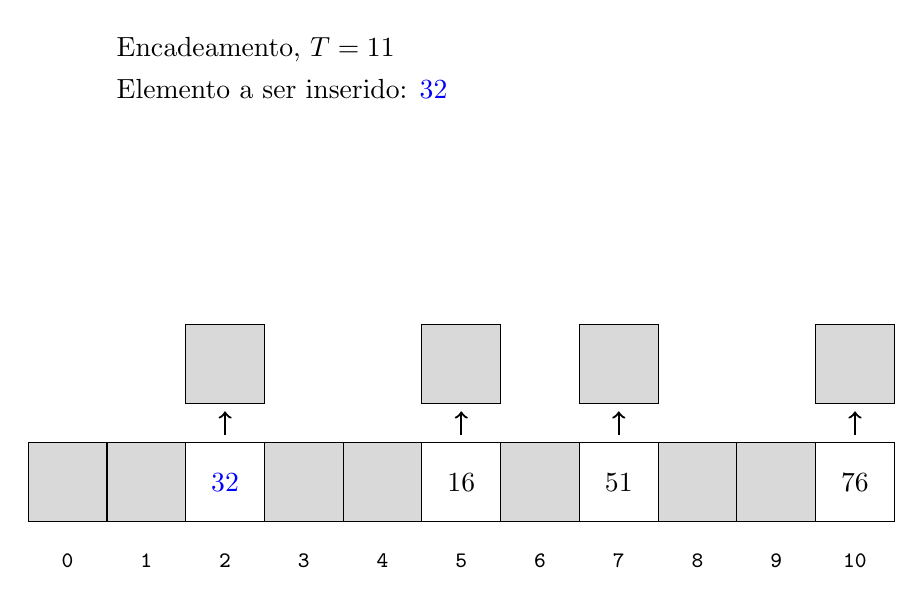
\begin{tikzpicture}
            \fill[gray!30] (0, 1) rectangle (11, 2);
            \draw[fill=white] (7, 1) rectangle (8, 2);
            \draw[fill=white] (5, 1) rectangle (6, 2);
            \draw[fill=white] (10, 1) rectangle (11, 2);
            \draw[fill=white] (2, 1) rectangle (3, 2);
            \draw (0, 1) grid (11, 2);

            \node at (0.5, 0.5) { \tt \footnotesize 0 };
            \node at (1.5, 0.5) { \tt \footnotesize 1 };
            \node at (2.5, 0.5) { \tt \footnotesize 2 };
            \node at (3.5, 0.5) { \tt \footnotesize 3 };
            \node at (4.5, 0.5) { \tt \footnotesize 4 };
            \node at (5.5, 0.5) { \tt \footnotesize 5 };
            \node at (6.5, 0.5) { \tt \footnotesize 6 };
            \node at (7.5, 0.5) { \tt \footnotesize 7 };
            \node at (8.5, 0.5) { \tt \footnotesize 8 };
            \node at (9.5, 0.5) { \tt \footnotesize 9 };
            \node at (10.5, 0.5) { \tt \footnotesize 10 };

            \draw[->, thick] (7.5, 2.1) -- (7.5, 2.4);
            \draw[fill=gray!30] (7, 2.5) rectangle (8, 3.5);
            \node at (7.5, 1.5) { \textcolor{black}{$51$} };

            \draw[->, thick] (5.5, 2.1) -- (5.5, 2.4);
            \draw[fill=gray!30] (5, 2.5) rectangle (6, 3.5);
            \node at (5.5, 1.5) { \textcolor{black}{$16$} };

            \draw[->, thick] (10.5, 2.1) -- (10.5, 2.4);
            \draw[fill=gray!30] (10, 2.5) rectangle (11, 3.5);
            \node at (10.5, 1.5) { \textcolor{black}{$76$} };

            \draw[->, thick] (2.5, 2.1) -- (2.5, 2.4);
            \draw[fill=gray!30] (2, 2.5) rectangle (3, 3.5);
            \node at (2.5, 1.5) { \textcolor{blue}{$32$} };

            \node[anchor=west] at (1, 7) { Encadeamento, $T = 11$ };
            \node[anchor=west] at (1, 6.5) { Elemento a ser inserido: \textcolor{blue}{$32$} };

        \end{tikzpicture}
    \end{figure}

\end{frame}

\begin{frame}{Exemplo de inserção utilizando encadeamento}

    \begin{figure}
        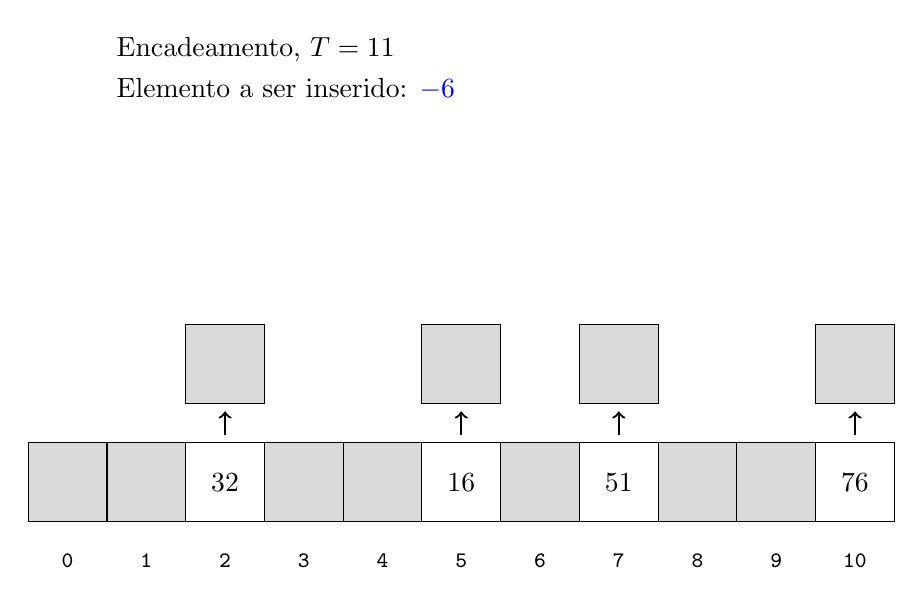
\begin{tikzpicture}
            \fill[gray!30] (0, 1) rectangle (11, 2);
            \draw[fill=white] (7, 1) rectangle (8, 2);
            \draw[fill=white] (5, 1) rectangle (6, 2);
            \draw[fill=white] (10, 1) rectangle (11, 2);
            \draw[fill=white] (2, 1) rectangle (3, 2);
            \draw (0, 1) grid (11, 2);

            \node at (0.5, 0.5) { \tt \footnotesize 0 };
            \node at (1.5, 0.5) { \tt \footnotesize 1 };
            \node at (2.5, 0.5) { \tt \footnotesize 2 };
            \node at (3.5, 0.5) { \tt \footnotesize 3 };
            \node at (4.5, 0.5) { \tt \footnotesize 4 };
            \node at (5.5, 0.5) { \tt \footnotesize 5 };
            \node at (6.5, 0.5) { \tt \footnotesize 6 };
            \node at (7.5, 0.5) { \tt \footnotesize 7 };
            \node at (8.5, 0.5) { \tt \footnotesize 8 };
            \node at (9.5, 0.5) { \tt \footnotesize 9 };
            \node at (10.5, 0.5) { \tt \footnotesize 10 };

            \draw[->, thick] (7.5, 2.1) -- (7.5, 2.4);
            \draw[fill=gray!30] (7, 2.5) rectangle (8, 3.5);
            \node at (7.5, 1.5) { \textcolor{black}{$51$} };

            \draw[->, thick] (5.5, 2.1) -- (5.5, 2.4);
            \draw[fill=gray!30] (5, 2.5) rectangle (6, 3.5);
            \node at (5.5, 1.5) { \textcolor{black}{$16$} };

            \draw[->, thick] (10.5, 2.1) -- (10.5, 2.4);
            \draw[fill=gray!30] (10, 2.5) rectangle (11, 3.5);
            \node at (10.5, 1.5) { \textcolor{black}{$76$} };

            \draw[->, thick] (2.5, 2.1) -- (2.5, 2.4);
            \draw[fill=gray!30] (2, 2.5) rectangle (3, 3.5);
            \node at (2.5, 1.5) { \textcolor{black}{$32$} };

            \node[anchor=west] at (1, 7) { Encadeamento, $T = 11$ };
            \node[anchor=west] at (1, 6.5) { Elemento a ser inserido: \textcolor{blue}{$-6$} };

        \end{tikzpicture}
    \end{figure}

\end{frame}

\begin{frame}{Exemplo de inserção utilizando encadeamento}

    \begin{figure}
        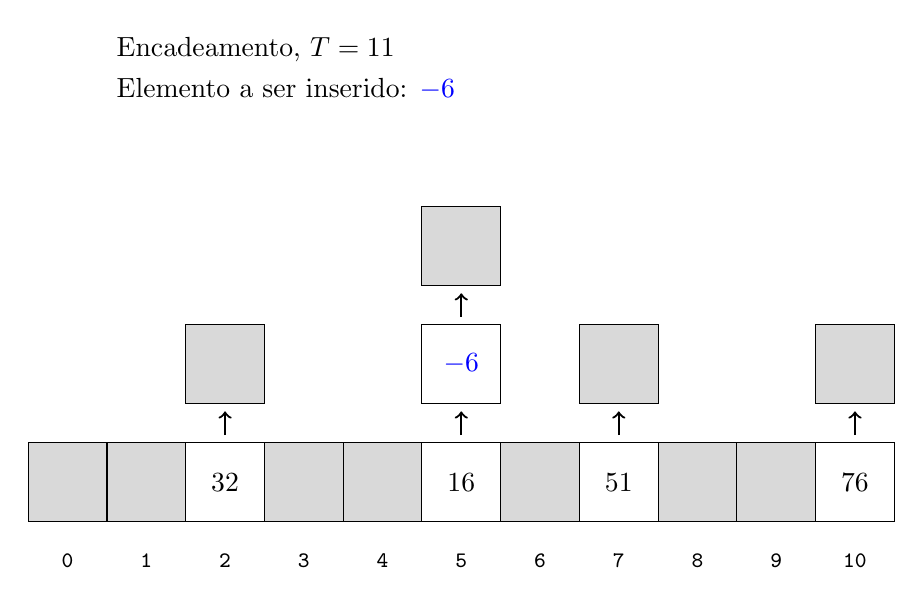
\begin{tikzpicture}
            \fill[gray!30] (0, 1) rectangle (11, 2);
            \draw[fill=white] (7, 1) rectangle (8, 2);
            \draw[fill=white] (5, 1) rectangle (6, 2);
            \draw[fill=white] (10, 1) rectangle (11, 2);
            \draw[fill=white] (2, 1) rectangle (3, 2);
            \draw (0, 1) grid (11, 2);

            \node at (0.5, 0.5) { \tt \footnotesize 0 };
            \node at (1.5, 0.5) { \tt \footnotesize 1 };
            \node at (2.5, 0.5) { \tt \footnotesize 2 };
            \node at (3.5, 0.5) { \tt \footnotesize 3 };
            \node at (4.5, 0.5) { \tt \footnotesize 4 };
            \node at (5.5, 0.5) { \tt \footnotesize 5 };
            \node at (6.5, 0.5) { \tt \footnotesize 6 };
            \node at (7.5, 0.5) { \tt \footnotesize 7 };
            \node at (8.5, 0.5) { \tt \footnotesize 8 };
            \node at (9.5, 0.5) { \tt \footnotesize 9 };
            \node at (10.5, 0.5) { \tt \footnotesize 10 };

            \draw[->, thick] (7.5, 2.1) -- (7.5, 2.4);
            \draw[fill=gray!30] (7, 2.5) rectangle (8, 3.5);
            \node at (7.5, 1.5) { \textcolor{black}{$51$} };

            \draw[->, thick] (5.5, 2.1) -- (5.5, 2.4);
            \draw (5, 2.5) rectangle (6, 3.5);
            \node at (5.5, 1.5) { \textcolor{black}{$16$} };

            \draw[->, thick] (10.5, 2.1) -- (10.5, 2.4);
            \draw[fill=gray!30] (10, 2.5) rectangle (11, 3.5);
            \node at (10.5, 1.5) { \textcolor{black}{$76$} };

            \draw[->, thick] (2.5, 2.1) -- (2.5, 2.4);
            \draw[fill=gray!30] (2, 2.5) rectangle (3, 3.5);
            \node at (2.5, 1.5) { \textcolor{black}{$32$} };

            \draw[->, thick] (5.5, 3.6) -- (5.5, 3.9);
            \draw[fill=gray!30] (5, 4) rectangle (6, 5);
            \node at (5.5, 3) { \textcolor{blue}{$-6$} };

            \node[anchor=west] at (1, 7) { Encadeamento, $T = 11$ };
            \node[anchor=west] at (1, 6.5) { Elemento a ser inserido: \textcolor{blue}{$-6$} };

        \end{tikzpicture}
    \end{figure}

\end{frame}

\begin{frame}{Exemplo de inserção utilizando encadeamento}

    \begin{figure}
        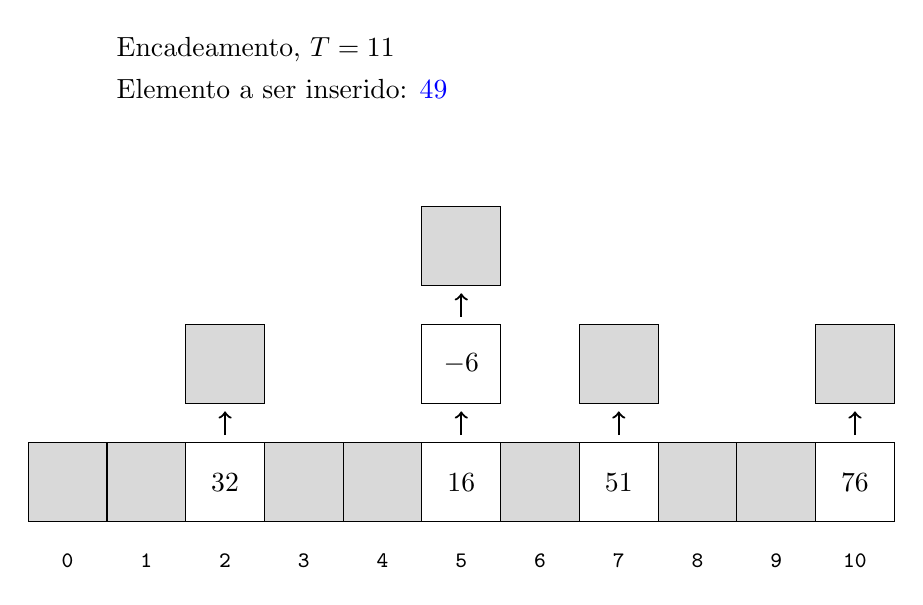
\begin{tikzpicture}
            \fill[gray!30] (0, 1) rectangle (11, 2);
            \draw[fill=white] (7, 1) rectangle (8, 2);
            \draw[fill=white] (5, 1) rectangle (6, 2);
            \draw[fill=white] (10, 1) rectangle (11, 2);
            \draw[fill=white] (2, 1) rectangle (3, 2);
            \draw (0, 1) grid (11, 2);

            \node at (0.5, 0.5) { \tt \footnotesize 0 };
            \node at (1.5, 0.5) { \tt \footnotesize 1 };
            \node at (2.5, 0.5) { \tt \footnotesize 2 };
            \node at (3.5, 0.5) { \tt \footnotesize 3 };
            \node at (4.5, 0.5) { \tt \footnotesize 4 };
            \node at (5.5, 0.5) { \tt \footnotesize 5 };
            \node at (6.5, 0.5) { \tt \footnotesize 6 };
            \node at (7.5, 0.5) { \tt \footnotesize 7 };
            \node at (8.5, 0.5) { \tt \footnotesize 8 };
            \node at (9.5, 0.5) { \tt \footnotesize 9 };
            \node at (10.5, 0.5) { \tt \footnotesize 10 };

            \draw[->, thick] (7.5, 2.1) -- (7.5, 2.4);
            \draw[fill=gray!30] (7, 2.5) rectangle (8, 3.5);
            \node at (7.5, 1.5) { \textcolor{black}{$51$} };

            \draw[->, thick] (5.5, 2.1) -- (5.5, 2.4);
            \draw (5, 2.5) rectangle (6, 3.5);
            \node at (5.5, 1.5) { \textcolor{black}{$16$} };

            \draw[->, thick] (10.5, 2.1) -- (10.5, 2.4);
            \draw[fill=gray!30] (10, 2.5) rectangle (11, 3.5);
            \node at (10.5, 1.5) { \textcolor{black}{$76$} };

            \draw[->, thick] (2.5, 2.1) -- (2.5, 2.4);
            \draw[fill=gray!30] (2, 2.5) rectangle (3, 3.5);
            \node at (2.5, 1.5) { \textcolor{black}{$32$} };

            \draw[->, thick] (5.5, 3.6) -- (5.5, 3.9);
            \draw[fill=gray!30] (5, 4) rectangle (6, 5);
            \node at (5.5, 3) { \textcolor{black}{$-6$} };

            \node[anchor=west] at (1, 7) { Encadeamento, $T = 11$ };
            \node[anchor=west] at (1, 6.5) { Elemento a ser inserido: \textcolor{blue}{$49$} };

        \end{tikzpicture}
    \end{figure}

\end{frame}

\begin{frame}{Exemplo de inserção utilizando encadeamento}

    \begin{figure}
        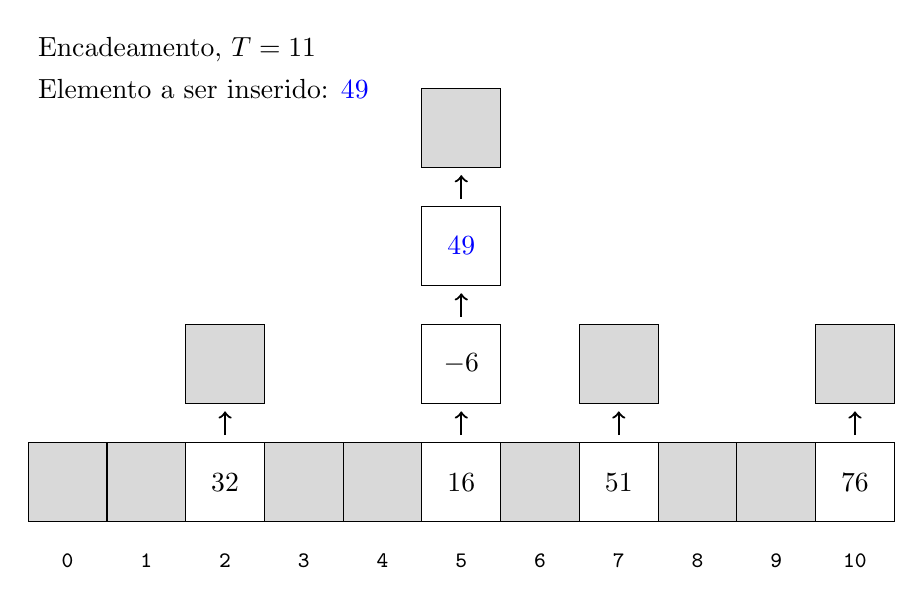
\begin{tikzpicture}
            \fill[gray!30] (0, 1) rectangle (11, 2);
            \draw[fill=white] (7, 1) rectangle (8, 2);
            \draw[fill=white] (5, 1) rectangle (6, 2);
            \draw[fill=white] (10, 1) rectangle (11, 2);
            \draw[fill=white] (2, 1) rectangle (3, 2);
            \draw (0, 1) grid (11, 2);

            \node at (0.5, 0.5) { \tt \footnotesize 0 };
            \node at (1.5, 0.5) { \tt \footnotesize 1 };
            \node at (2.5, 0.5) { \tt \footnotesize 2 };
            \node at (3.5, 0.5) { \tt \footnotesize 3 };
            \node at (4.5, 0.5) { \tt \footnotesize 4 };
            \node at (5.5, 0.5) { \tt \footnotesize 5 };
            \node at (6.5, 0.5) { \tt \footnotesize 6 };
            \node at (7.5, 0.5) { \tt \footnotesize 7 };
            \node at (8.5, 0.5) { \tt \footnotesize 8 };
            \node at (9.5, 0.5) { \tt \footnotesize 9 };
            \node at (10.5, 0.5) { \tt \footnotesize 10 };

            \draw[->, thick] (7.5, 2.1) -- (7.5, 2.4);
            \draw[fill=gray!30] (7, 2.5) rectangle (8, 3.5);
            \node at (7.5, 1.5) { \textcolor{black}{$51$} };

            \draw[->, thick] (5.5, 2.1) -- (5.5, 2.4);
            \draw (5, 2.5) rectangle (6, 3.5);
            \node at (5.5, 1.5) { \textcolor{black}{$16$} };

            \draw[->, thick] (10.5, 2.1) -- (10.5, 2.4);
            \draw[fill=gray!30] (10, 2.5) rectangle (11, 3.5);
            \node at (10.5, 1.5) { \textcolor{black}{$76$} };

            \draw[->, thick] (2.5, 2.1) -- (2.5, 2.4);
            \draw[fill=gray!30] (2, 2.5) rectangle (3, 3.5);
            \node at (2.5, 1.5) { \textcolor{black}{$32$} };

            \draw[->, thick] (5.5, 3.6) -- (5.5, 3.9);
            \draw (5, 4) rectangle (6, 5);
            \node at (5.5, 3) { \textcolor{black}{$-6$} };

            \draw[->, thick] (5.5, 5.1) -- (5.5, 5.4);
            \draw[fill=gray!30] (5, 5.5) rectangle (6, 6.5);
            \node at (5.5, 4.5) { \textcolor{blue}{$49$} };

            \node[anchor=west] at (0, 7) { Encadeamento, $T = 11$ };
            \node[anchor=west] at (0, 6.5) { Elemento a ser inserido: \textcolor{blue}{$49$} };

        \end{tikzpicture}
    \end{figure}

\end{frame}
